\chapter{Marco Referencial}
\section{Marco conceptual}
\subsection{Descubrimiento del conocimiento en bases de datos (KDD)}
En \cite{key-60} se define como: \begin{quote} Es el proceso de utilizar la información contenida en los sistemas de almacenamientos de datos para identificar patrones significativos, validos, novedosos, potencialmente útiles y comprensibles para el usuario. El proceso global consiste en transformar información de bajo nivel en conocimiento de alto nivel. El proceso KDD es interactivo e iterativo conteniendo los siguientes pasos: comprender el dominio de aplicación, extraer la base de datos objetivo, preparar los datos, minería de datos, interpretación y utilizar el conocimiento descubierto \end{quote}.
\subsection{Minería de datos}
En \cite{key-60} se define como: \begin{quote} Es un campo interdisciplinar con el objetivo general de predecir las salidas y revelar relaciones en los datos. Las tareas propias de la minería de datos pueden ser descriptivas, (i.e. descubrir patrones interesantes o relaciones describiendo los datos), o predictivas (i.e. clasificar nuevos datos basándose en los anteriormente disponibles). Para ello se utilizan herramientas automáticas que emplean algoritmos sofisticados para descubrir principalmente patrones ocultos, asociaciones, anomalías, y/o estructuras de la gran cantidad de datos almacenados en los Data Warehouses u otros repositorios de información, y filtran la información necesaria de las grandes bases de datos \end{quote}.
\subsection{ICFES}
Instituto Colombiano para la Evaluación de la Educación, entidad especializada en ofrecer servicios de evaluación de la educación en todos sus niveles, y en particular apoyar al Ministerio de Educación Nacional en la realización de los exámenes de Estado y en adelantar investigaciones sobre los factores que inciden en la calidad educativa, para ofrecer información pertinente y oportuna para contribuir al mejoramiento de la calidad de la educación en Colombia \cite{key-80}.
\subsection{Prueba Saber 11\degree}\label{sec:saber11}
Antes conocida como Examen del ICFES, es un examen de estado que evalúa a los estudiantes que están terminando su ciclo de Educación Media. La prueba tiene como finalidad apoyar los procesos de selección y admisión que realizan las instituciones de Educación Superior. Además de este propósito, la prueba busca:
\begin{itemize}
\item Brindar al estudiante información que contribuya a la selección de
su opción profesional. 
\item Proporcionar información a las instituciones de educación básica y
media sobre el desempeño de los estudiantes. 
\item Contribuir al desarrollo de estudios de tipo cultural, social y educativo. 
\item Servir de criterio para otorgar beneficios educativos. 
\end{itemize}
Las áreas académicas evaluadas actualmente por la prueba Saber 11\degree \ son:
\begin{itemize}
\item Lenguaje 
\item Matemáticas 
\item Biología 
\item Química 
\item Física 
\item Filosofía 
\item Ciencias sociales 
\item Inglés 
\item COMPONENTE FLEXIBLE (solo se presenta una de las siguientes opciones)
\begin{itemize}
\item Profundización en lenguaje 
\item Profundización en matemáticas 
\item Profundización en biología 
\item Profundización en ciencias sociales 
\item Interdisciplinar violencia y sociedad 
\item Interdisciplinar medio ambiente
\end{itemize}
\end{itemize}
\subsection{Data Warehouse}
Es un repositorio de datos operacionales seleccionados y adaptados subjetivamente, que puede responder consultas de tipo ad hoc, estadísticas o analíticas. Está situado en el centro de los sistemas de apoyo a la toma de decisiones de una organización y contiene datos históricos, resumidos y detallados de esta. Es esencial para una inteligencia de negocios efectiva, para la formulación e implementación de estrategias donde la gran cantidad de datos requieren ser procesados de manera rápida para comprender su significado e impacto. Permite una fácil organización y mantenimiento de los datos para una rápida recuperación y análisis de la manera en que sean requeridos \cite{key-90}.
\subsection{Data Mart}
Desde un Data Warehouse, los datos fluyen hacia los departamentos de la organización, que personalizan la información almacenada para que sea útil en los sistemas de información de cada uno de ellos. Estos componentes individuales con características personalizadas son conocidos como Data Mart. En otras palabras, es un cuerpo de datos de un sistema de información, que posee la estructura fundamental de un Data Warehouse, es una subsección de una Data Warehouse y más popular que este \cite{key-90}.
\section{Antecedentes o Estado del Arte}
En el área de la educación, los trabajos presentados a continuación se orientaron a encontrar posibilidades de bajos rendimiento académicos y así lograr conocer perfiles o factores que hacen que los estudiantes no logren las metas propuestas en sus estudios. Este trabajo de grado también se orientó a encontrar estas posibilidades de bajos rendimientos, pero no aplicado a estudiantes de universidades, sino a los estudiantes que presentan la prueba Saber 11\degree.

También se observó la variedad de algoritmos utilizados para construir los clasificadores, en algunos trabajos se utilizó más de un algoritmo para lograr encontrar comparaciones de rendimiento y mejores niveles de precisión con cada algoritmo. En este trabajo se evaluaron distintos algoritmos para la construcción de clasificadores, con el fin de encontrar información sobre cómo se comportan con la cantidad de datos usados y con la estructura que posean estos datos.

En este trabajo se utilizaron bases de datos que contenían más de 5 millones de registros\footnote{\url{ftp://ftp.icfes.gov.co/SABER11/SB11-FTP_Algunos_Totales_de_Control-v1-1.pdf}}, recolectados a lo largo de 11 años y que presentan una gran variación en la integridad de los atributos de estos registros. Por eso este trabajo centró su primera parte en la homogeneización de estas bases de datos. En los trabajos revisados, la cantidad de datos utilizados en los procesos de investigación, no eran tantos como los que se utilizaron en este trabajo.

En conclusión los trabajos aquí presentados sirvieron de base para la realización de este trabajo, ya que sus fases de investigación fueron las mismas en la mayoría de los trabajos, iguales a las que se aplicaron en este trabajo. Además, los resultados obtenidos en ellos, muestran la utilidad de la construcción de clasificadores para predecir resultados de estudiantes en exámenes o procesos de su vida académica.
\subsection{Detección de patrones de bajo rendimiento académico y deserción estudiantil con técnicas de minería de datos \cite{key-100}}
Su objetivo fue determinar en la comunidad universitaria perfiles de bajo rendimiento académico y deserción estudiantil aplicando técnicas de descubrimiento del conocimiento, a partir de los datos almacenados en las bases de datos durante los últimos 15 años. Este proceso se apoyó con TariyKDD\footnote{\url{http://developer.berlios.de/projects/tariykdd/}}, una herramienta de minería de datos de distribución libre. Aunque el trabajo de investigación este orientado a detectar bajos rendimientos de estudiantes en la universidad, su proceso de investigación es similar al que se espera llevar en este proyecto, por lo tanto sirve de guía para el desarrollo de este. Además de que la información utilizada para predecir el comportamiento académico de los estudiantes se basa en información socio-económica, que es la misma con la que se cuenta en las bases de datos del ICFES para construir el clasificador.

Este trabajo desarrolló de manera organizada y bien estructurada, cada uno de los pasos planteados en \cite{key-50}. El algoritmo de minería de datos utilizado fue arboles de clasificación con C4.5 \cite{key-50, key-70}, los resultados entregados por esta investigación mostraron cuales eran los perfiles de los estudiantes que podrían prever un bajo rendimiento.
La investigación se realizó en la Universidad de Nariño de Colombia. Las bases de datos recolectadas contenían información sobre el desempeño académico e información personal de 46173 estudiantes, acumuladas durante 15 años.

Inicialmente se contaba con 69 atributos en las bases de datos que describían las características de los estudiantes, pero después de pasar por el proceso de limpieza y transformación de los datos, y utilizando TariyKDD para seleccionar los atributos más relevantes, se llegó a una lista de 26 atributos y una cantidad de registros de 20329.

Finalmente, se aplicaron las técnicas de minería de datos para clasificación, en este caso el algoritmo C4.5 y se obtuvieron las reglas que indicaban que tipo de situaciones personales de un estudiante podrían llevar a obtener un bajo rendimiento en la universidad. Unos ejemplos de las reglas obtenidas son:
\begin{itemize}
\item Si el estrato socioeconómico es 2, el ponderado de exámenes de estado ICFES está entre 50 y 70, es del Sur de Nariño, está en primer semestre y pertenece a la facultad de Ciencias Humanas, entonces su rendimiento es Bajo. El 68\% con estas características se clasifican de esta manera. 
\item Si la edad de ingreso es menor o igual a 18 años, el estrato socioeconómico es 2, género masculino, el ponderado ICFES está entre 50 y 70, vive con la familia, es del Sur de Nariño, está en primer semestre, está en la facultad de Ciencias Naturales y Matemáticas, entonces su rendimiento es Bajo. El 67\% con estas características se clasifican de esta manera. 
\end{itemize}
\subsection{Minería de datos en la educación \cite{key-110}}
En este documento se describe el uso de la minería de datos aplicada a entornos educativos y su uso pedagógico. De manera muy clara y especifica brinda una vista de cómo se debe realizar un proceso de minería de datos en educación y su importancia.

Además muestra un ejemplo: ``Identificación de características de fracasos escolares en institutos''. En este se usan arboles de decisión porque permiten encontrar cuales son las variables que tienen mayor relación con la variable que se desea predecir. El algoritmo de árboles de decisión utilizado fue CHAID \cite{key-120} (Chi-Squared Automatic Interaction Detection). CHAID realiza comparaciones en pares para encontrar la variable de predicción más altamente relacionada con la variable raíz. En sistemas de muchas variables, tener esta función implementada en un ordenador es esencial para procesar amplios conjuntos de datos (Big Data) \cite{key-110}. El resultado entregado fue un árbol, el cual se debió analizar para determinar su información.
\subsection{Minería de datos: predicción de la deserción escolar mediante el algoritmo de árboles de decisión y el algoritmo de los k vecinos más cercanos \cite{key-130}}
Se aplicaron técnicas de minería de datos para buscar conocer previamente si los estudiantes eran propensos a abandonar su carrera en la Universidad Tecnológica de Izúcar de Matamoros, México, tomando como base de análisis los datos del estudio socioeconómico del EXANI-II\footnote{\url{http://www.ceneval.edu.mx/ceneval-web/content.do?page=1738}}, elaborado por el CENEVAL\footnote{\url{http://www.ceneval.edu.mx/ceneval-web/content.do?page=1702}}, mismo que se aplica desde el año 2003 en la institución. Para esta investigación se utilizaron específicamente dos algoritmos: el algoritmo de árboles de clasificación C4.5 y el algoritmo de los k vecinos más cercanos \cite{key-70}.

En el proceso de transformación de los datos, el más largo en muchos de los trabajos que se realizan, incluyendo este, se modificó e integró toda la información encontrada en distintos formatos de almacenamiento, además no tenía un estructura clara, porque constaba de información de estudiantes de 14 cuatrimestres, por supuesto en cada registro no se realizaban las mismas preguntas, además de que muchas de estas se pueden responder como ``No lo sé'', después de superar esta etapa y aplicar los algoritmos previstos, se encontró que el algoritmo de los k vecinos más cercanos funciona bien con pocos datos (477 instancias), pero al momento de probarlo con 6525 instancias, el algoritmo C4.5, tuvo resultados más confiables (98,98\%).

Aquí también se realizó la creación de una herramienta que pueda ser accedida por cualquier usuario y le informa sobre la probabilidad de que un estudiante deserte. Los resultados mostraron que la edad, la situación económica y el nivel de inglés, tienen fuerte relación con que el estudiante deserte de la universidad.
\subsection{Modelo predictivo para la determinación de causas de reprobación mediante minería de datos \cite{key-140}}
En este trabajo, realizado en la Universidad Tecnológica de Puebla, México, se llevó a cabo el análisis de los datos que permitirán generar un modelo que ayude a predecir, desde que los alumnos ingresan a la Universidad, las causas que los llevarán a reprobar, así como las materias con mayor riesgo de ser reprobadas.

El algoritmo de clasificación utilizado fue C4.5, y se recolectaron datos con información de todas las carreras ofrecidas por la universidad. Este proceso de nuevo fue demorado, porque sus fuentes de almacenamiento poseían distintas estructuras y no existía una homogeneidad en los datos.

Los resultados obtenidos mostraron que de las 157 materias distintas que ofrece la universidad en sus carreras, 64 materias tienen un porcentaje de reprobación menor a 40\% y por lo tanto no generan un árbol de predicción. En las materias con un porcentaje mayor al 50\% se determinó que el factor principal de reprobación es el profesor que imparte la materia y también la edad de los estudiantes.
\subsection{La metodología del Data Mining. Una aplicación al consumo de alcohol en adolescentes \cite{key-150}}
Aunque en esta investigación el objetivo no estaba focalizado en descubrir conocimiento en el área de la educación. Es un trabajo interesante el cual sirvió de guía en este trabajo de grado, ya que en él se realizó la construcción de 3 algoritmos distintos de predicción: redes neuronales, arboles de decisión y Naive Bayes \cite{key-50}.

El trabajo se centra en demostrar la importancia que tiene el descubrimiento del conocimiento en bases de datos al momento de predecir comportamientos en distintas áreas como educación, finanzas, comercio, telecomunicaciones, salud, entre otras.

Estos algoritmos fueron aplicados en un conjunto de datos que contenía 7030 registro que informaban sobre el consumo de alcohol en jóvenes de entre 14 y 18 años con una cantidad de 20 variables que incluían información de la personalidad como los constructos de autoestima, impulsividad, conducta antisocial y búsqueda de sensaciones.

Los mejores resultados se obtuvieron con el modelo construido con redes neuronales, 64,1\% de precisión al momento de predecir si un joven consumía o no alcohol. Los otros resultados fueron una precisión de 62,3\% con árboles de decisión usando el algoritmo CART \cite{key-50} y una precisión de 59,9\% usando Naive Bayes.
\section{Marco Teórico}
\subsection{Metodología para el proceso del descubrimiento del conocimiento (KDD)}
Para la realización de este trabajo se utilizó el conjunto de fases presentadas en \cite{key-50} donde establece que: ``Este proceso es iterativo e interactivo. Es iterativo ya que la salida de alguna de las fases puede hacer volver a pasos anteriores y porque a menudo son necesarias varias iteraciones para extraer conocimiento de alta calidad. Es interactivo porque el usuario (experto en el dominio del problema) interviene en la toma de muchas decisiones''.

La teoría del proceso del desarrollo de un proyecto de descubrimiento del conocimiento en bases de datos, define los siguientes pasos:
\begin{figure}[H]
\begin{centering}
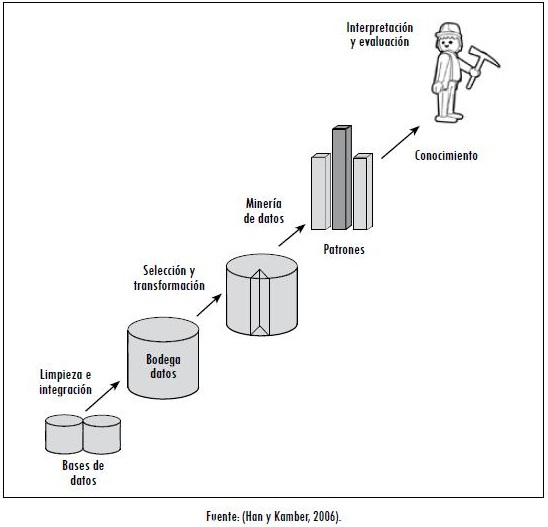
\includegraphics[scale=0.5]{v13n1a07-3}
\par\end{centering}
\caption{Proceso de descubrimiento del conocimiento en bases de datos.}
\end{figure}
\subsubsection{Selección (\emph{Extraction}) \cite{key-50,key-100}}
En esta etapa del proceso, es donde se investigan las fuentes, en las cuales se podrán encontrar los datos que me servirán para general un almacén de datos con información útil. Se recolectan todos los datos obtenidos en estas fuentes y se organizan en bases de datos que se usaran para la etapa de transformación.

Comúnmente en los trabajos orientados a la academia \cite{key-100, key-110, key-130, key-140}, estos datos son la información de los estudiantes de la institución a lo largo del tiempo. Los datos pueden incluir información acerca de la situación socio-económica del estudiante, sus notas, su entorno académico, información familiar, entre muchas otras que defina la institución que es importante recolectar.

En \cite{key-140}, donde se buscaba encontrar las reglas que indicaran si un estudiante era propenso a reprobar una materia, se seleccionaron como datos útiles: calificaciones por área del examen de admisión EXANI II, datos relevantes del estudio socio-económico, calificación del test de intereses vocacionales (KUDER), calificación del test de coeficiente intelectual (RAVEN), estilos de aprendizaje, evaluación a profesores, asignaturas cursadas y su promedio por cuatrimestre.
\subsubsection{Transformación (\emph{Transformation}) \cite{key-50,key-100}}
En esta etapa el proceso se basa en realizar primero una limpieza de los datos, la limpieza permite obtener datos sin valores nulos o anómalos, además se estandarizan los datos para que sean del mismo tipo. 

Para eliminar los datos nulos, se puede omitir este atributo o en algunos casos, cuando no son muchos los registros carentes de este valor, se pueden aplicar técnicas estadísticas como la media para insertar un valor valido y así no eliminar el registro o el atributo de la base de datos.

Estos procesos de limpieza, integración y agregación de los datos, entregan como resultado una base de datos modificada con los atributos relevantes en los registros, para responder al objetivo de la investigación, muchas veces esto genera que la cantidad de registros que se tenían inicialmente, se disminuya significativamente. Pero esto permitirá obtener resultados mucho más confiables, ya que no habrá datos que generen conflictos a la hora de generar clasificaciones con respecto a algunos atributos.
\subsubsection{Carga (\emph{Load}) \cite{key-50,key-100}}
En esta etapa se transfieren los datos procesados en las fases anteriores al medio de almacenamiento escogido por el equipo de desarrollo. Estos medios de almacenamiento pueden ser bases de datos, Data Warehouse, Data Mart, entre otros.
\subsubsection{Minería de datos \cite{key-50,key-100}}
El objetivo de esta etapa es la búsqueda y descubrimiento de patrones insospechados y de interés utilizando diferentes técnicas de descubrimiento tales como clasificación, clustering, patrones secuenciales, asociación, entre otras \cite{key-100}. Las diferentes técnicas utilizadas pertenecen a campos como la inteligencia artificial y estadísticas. Algunos algoritmos usados comúnmente son: arboles de decisión C4.5, ID3 \cite{key-160} y CHAID (Detección Automática de Interacción basada en Chi-Cuadrado), algoritmo de los k vecinos más cercanos, Naive Bayes, redes neuronales, algoritmo de reglas de asociación Apriori, algoritmo de inducción de reglas como el Prism, diferentes versiones de algoritmos evolutivos, programación genética basada en gramática.
\subsubsection{Interpretación y evaluación de los resultados \cite{key-50,key-100}}
En esta etapa se interpretan los patrones descubiertos y posiblemente se retorna a los anteriores pasos o etapas para posteriores iteraciones. Esta etapa puede incluir la visualización de los patrones extraídos, la remoción de los patrones redundantes o irrelevantes y la traducción de los patrones útiles en términos que sean entendibles para el usuario final de la aplicación \cite{key-100}.
\subsection{Clasificación}
En la minería de datos, probablemente la tarea más popular por su objetivo es la clasificación. En esta tarea el objetivo es construir una función que permita, usando los atributos de una instancia, conocer la clase a la cual puede pertenecer la instancia. Para la construcción de los clasificadores se utiliza un conjunto de datos de entrenamiento, los cuales contiene un grupo de atributos predictores y un atributo a predecir, normalmente conocido como la clase a predecir. \\
Formalmente, en \cite{key-70} se define como la tarea de aproximar una \emph{función objetivo} desconocida, que describe cómo instancias del problema deben ser clasificadas
de acuerdo a un experto en el dominio, \begin{quote}$\Phi:I\times C\rightarrow\left\{ T,F\right\} $\end{quote}
 por medio de una función llamada el \emph{clasificador}, \begin{quote}
$\Theta:I\times C\rightarrow\left\{ T,F\right\} $
\end{quote} 
 donde \begin{quote}
 $C=\left\{ c_{1},...,c_{|c|}\right\} $ es un conjunto de categorías predefinido\end{quote}
 e \begin{quote}\emph{I} es un conjunto
de instancias del problema\end{quote} Comúnmente cada instancia $i_{j}\epsilon I$
es representada como una lista $A=\left\{ a_{1},a_{2},...,a_{|A|}\right\} $
de valores característicos, conocidos como \emph{atributos}, i.e.
$i_{j}=\left\{ a_{1},a_{2},...,a_{|A|j}\right\} $. \\Si \begin{quote}$\Phi:i_{j}\times c_{i}\rightarrow T$,
entonces es llamado un ejemplo positivo de $c_{i}$ \end{quote} mientras si \begin{quote}$\Phi:i_{j}\times c_{i}\rightarrow F$
éste es llamado un ejemplo negativo de $c_{i}$\end{quote}

Para generar automáticamente el clasificador de $c_{i}$ es necesario
un proceso inductivo, llamado el \emph{aprendizaje}, el cual por observar
los atributos de un conjunto de instancias preclasificadas bajo $c_{i}$
o $\bar{c_{i}}$, adquiere los atributos que una instancia no vista
debe tener para pertenecer a la categoría. Por tal motivo, en la construcción
del clasificador se requiere la disponibilidad inicial de una colección
$\Omega$ de ejemplos tales que el valor de $\Phi\left(i_{j},c_{i}\right)$
es conocido para cada $\left\langle i_{j},c_{i}\right\rangle \epsilon\Omega\times C$.
A la colección usualmente se le llama \emph{conjunto de entrenamiento}
$\left(Tr\right)$.
\subsection{Evaluación de clasificadores}
Al momento de evaluar un clasificador, lo que se busca es conocer como es clasificada cada una de las instancias de un conjunto de evaluación. En estas instancias se conoce la clase a la cual pertenecen. El clasificador, procesa el conjunto de evaluación y retorna la clase a la que cada instancia debería pertenecer según los atributos predictores que contiene.\\
Usando las clasificaciones reales y las retornadas después de la evaluación, se generan 2 valores de evaluación de la calidad del clasificador. Estos 2 valores son Precisión y Exhaustividad (Presicion and Recall).\\
La precisión es la fracción de instancias correctamente clasificadas en una clase y la exhaustividad en la fracción de instancias de una clase que se clasificaron correctamente. \cite{key-280}\\
Teniendo que:
\begin{center}
$A=Conjunto\ de\  instancias\  de\  la\  clase\  X\  en\  el\  conjunto\  de\  evaluaci\acute{o}n$

$B=Conjunto\  de\  instancias\  clasificadas\  en\  la\  clase\  X\  por\  el\  clasificador$
\end{center}
Entonces
\begin{center}
$Presici\acute{o}n=\frac{|A\cap B|}{|B|}$

$Recall=\frac{|A\cap B|}{|A|}$
\end{center}
Cuanto más cerca estén estos valores a 1, mejor será la calidad del clasificador.
\subsection{Generador de árboles de decisión C4.5}
Un árbol de decisión es un conjunto de condiciones organizadas en una estructura jerárquica. De tal manera que la decisión final se puede tomar siguiendo las condiciones desde la raíz hasta alguna de las hojas\cite{key-170}.

El problema de la construcción de un árbol puede ser explicado de una manera recursiva. Primero se selecciona un atributo para ser ubicado en la raíz del árbol, y se crea una rama por cada posible valor que puede tomar este atributo. Esto divide el conjunto de datos de entrenamiento en distintas secciones con cada valor del nodo raíz. Y el proceso se repite de manera recursiva por cada una de las nuevas ramas, usando las instancias que están presentes en cada nuevo nodo. La condición de parada es cuando todas las instancias en un nodo tienen la misma clasificación\cite{key-210}.
\begin{figure}[H]
\begin{centering}
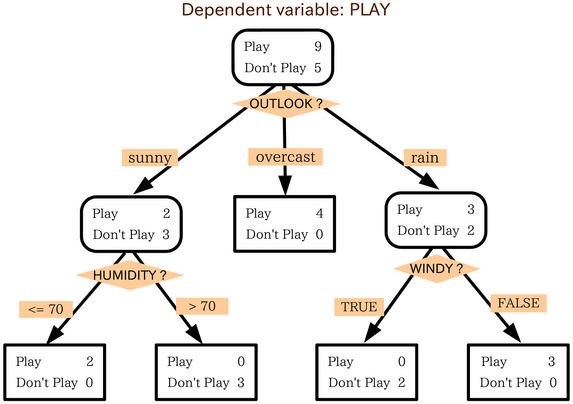
\includegraphics[scale=0.6]{c45}
\par\end{centering}
\caption{Representación gráfica de un árbol de decisión.}
\end{figure}
El problema de decidir que atributo debe ser ubicado en cada nodo se resuelve usando el factor de ganancia de información. En cada iteración se evalúa la ganancia de información que genera cada uno de los atributos y se selecciona el que obtenga un mayor valor. El valor de ganancia de información es calculado usando Gain Ratio.

Teniendo un conjunto \emph{S} de instancias, y \emph{frec($C_{i},S$)
}que es el número de casos de \emph{S} que pertenecen a la clase $C_{i}$
y $\left|S\right|$es el número de instancias en el conjunto. Entonces
la entropía de \emph{S }es:
\begin{center}
$H(S)=-\overset{k}{\underset{i=1}{\sum}}(\frac{frec(C_{i},S)}{|S|}*log_{2}(\frac{frec(C_{i},S)}{|S|}))$
\end{center}

Después se procede a encontrar la entropía de cada uno de los atributos de las instancias. Posteriormente, conociendo la entropía de cada subconjunto $\left|S\right|$ ($S_{j}$ es el subconjunto de instancias que
tienen igual valor en el atributo que se desea evaluar) se calcula
la ganancia de información que cada atributo genera.
\begin{center}
$H_{X}(S)=\overset{n}{\underset{j=1}{\sum}}(\frac{|S_{j}|}{|S|}*H(S_{j}))$ Entropía del atributo \emph{X} en el conjunto \emph{S}.

$G(X)=H(S)-H_{x}(S)$ Ganancia de información del atributo \emph{X}.
\end{center}

Se selecciona el atributo con mayor ganancia para ser ubicado en el
nodo que se está iterando, y se procede a calcular el siguiente nodo.
Las siguientes iteraciones no tendrán en cuenta en las instancias
los atributos que han ido siendo seleccionados previamente\cite{key-290}.
\subsection{K vecinos más cercanos}
La regla del vecino más cercano es simple, este asigna a la instancia
que se quiere clasificar, la clase del ejemplo más próximo utilizando
una función de distancia. Esta función usualmente es la función de
distancia Euclidiana, aunque una alternativa también frecuentemente
usada es la función de distancia Manhattan.

El problema con esta sencilla manera de clasificar las instancias,
es que toma mucho tiempo comparar, cada una de las instancias de entrenamiento
con la instancia a clasificar, para determinar cuál es la más cercana.
La manera de reducir el tiempo que toma esta comparación es representando
los datos de entrenamiento como un árbol, este árbol es llamado un
kD-tree\cite{key-220}, porque almacena un grupo de
puntos en un espacio k-dimensional. Siendo k el número de atributos
de las instancias.

El uso de los kD-tree ha ayudado a solucionar el problema de la comparación
uno por uno, ya que el árbol divide el espacio en dimensiones que
agrupan instancias con atributos similares, así cada evaluación no
debe compararse contra cada instancia, sino que se compara contra
las dimensiones, y se asigna a la clase de la dimensión con la que
tuvo una mayor similitud\cite{key-210}.

Este algoritmo tiene 3 elementos principales: el conjunto de instancias
de entrenamiento \emph{S}, una métrica para calcular la distancia
entre los objetos $d(x_{i},x')$ y el valor de vecinos mas
cercanos \emph{k}. 

Para clasificar una nueva instancia $z=(x',y')$ el algoritmo calcula
las distancias con las instancias de entrenamiento $(x,y)\epsilon S$
para determinar la lista de vecinos más cercanos. \emph{x} representa
el conjunto de atributos predictores de una instancias e \emph{y} representa
la clase de la instancia.

Una vez se tiene la lista de los vecinos más cercanos se selecciona
la clase de mayor frecuencia entre estos:
\begin{center}
$Clase\, Mayoritaria=y'=\underset{v}{argmax}\underset{(x_{i},y_{i})\epsilon S_{z}}{\sum}I(v,y_{i})$
\end{center}

donde \emph{v} es el valor de la clase, $y_{i}$ es el valor de la
clase del \emph{i}-ésimo vecino de la lista, $S_{z}$ es el conjunto
de las distancias entre las instancias de entrenamiento y la instancia
de evaluación \emph{z} y \emph{I(a,b)} es una función que retorna
1 si \emph{a} y \emph{b} son iguales, 0 si no\cite{key-300, key-180}.
\begin{figure}[H]
\begin{centering}
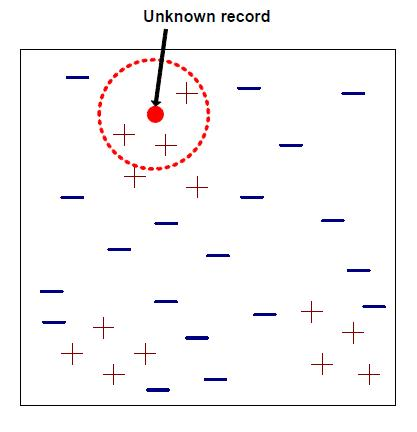
\includegraphics[scale=0.6]{knn}
\par\end{centering}
\caption{En esta representación, si k=3 el algoritmo retornará la clase B pero si k=6 el algoritmo retornará la clase A. Ya que se selecciona la clase mayoritaria entre los vecinos cercanos.}
\end{figure}
\subsection{Naive Bayes}
Los métodos bayesianos combaten uno de los problemas que poseen las técnicas de minería de datos, el manejo de la incertidumbre. Evitan este problema utilizando la teoría de la probabilidad para cuantificar la incertidumbre.

La inducción de modelos probabilísticos a partir de los datos conocidos, permite que se realice un razonamiento sobre los nuevos datos a observar. Además de que puede calcular la probabilidad asociada a cada una de las hipótesis. Y permite actualizar la creencia en un conjunto de hipótesis, cada que se estudia una nueva instancia, es decir con cada nueva instancia, su probabilidad mejora ya que es acumulativa\cite{key-230}.

El fundamento principal del clasificador Naive Bayes es la suposición de que todos los atributos son independientes conocido el valor de la clase. Esto da lugar a un modelo grafico probabilístico donde la raíz es la clase y todos los atributos son hijos de este nodo.

Teniendo en cuenta estos conceptos, el teorema de Bayes es representado por:
\begin{center}
$P(h|O)=\frac{P(O|h)*P(h)}{P(O)}$
\end{center}
Que indica la probabilidad de que una hipótesis \emph{h} suceda, teniendo en cuenta un conjunto de observaciones \emph{O}.

En un problema de clasificación el conjunto de observaciones es $O=\{A_{1},A_{2},...,A_{n}\}$ y la hipótesis \emph{h} es cada una de las clases posibles $h=\{c_{1},c_{2},...,c_{n}\}$. Se debe calcular la probabilidad de cada una de las clases en el conjunto \emph{h} y seleccionar la que entregue el valor más alto.
\begin{center}
$C_{MAP}=\underset{c\epsilon h}{arg\, max}\frac{P(O|c)*P(c)}{P(O)}=\underset{c\epsilon h}{arg\, max}P(O|c)*p(c)$
\end{center}
\begin{quote}
{*}MAP = Máximum A Posteriori, valor de probabilidad máxima obtenida después de calcular todas las clases en el conjunto \emph{h}.
\end{quote}
Teniendo en cuenta que Bayes supone que cada atributo es independiente,
entonces la probabilidad puede calcularse de la siguiente manera:
\begin{center}
$C_{MAP}=\underset{c\epsilon h}{arg\, max}P(c)*\overset{|O|}{\underset{i=1}{\Pi}}P(A_{i}|c)$
\end{center}
La probabilidad de cada uno de los atributos viene dada por el número
de instancias en las cuales el atributo $A_{i}$ toma el valor $a_{i}$y
la clase \emph{C} toma el valor $c_{i}$ sobre la cantidad de veces
que la clase \emph{C} toma el valor $c_{i}$\cite{key-50, key-190}.
\begin{center}
$P(a_{i}|c_{i})=\frac{frec(a_{i},c_{i})}{frec(c_{i})}$
\end{center}
De esta manera el algoritmo Naive Bayes se entrena y es capaz de clasificar
una nueva instancia.
\begin{figure}[H]
\begin{centering}
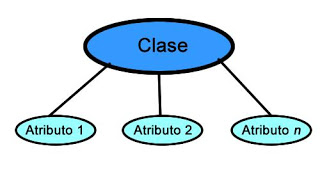
\includegraphics[scale=0.6]{nive}
\par\end{centering}
\caption{Representación gráfica del algoritmo Naive Bayes.}
\end{figure}
\subsection{Funciones de base radial}
Las redes neuronales artificiales (RNA) tienen distintas aplicaciones, entre ellas se encuentra la clasificación \cite{key-250}. Su objetivo es tratar de emular la capacidad humana de procesar información. 

Las RNA pueden ser entrenadas usando métodos de aprendizaje supervisado o no supervisado \cite{key-240}. Una de las redes encontradas en el aprendizaje supervisado es la red de Funciones de Base Radial. Las redes RBF constan de 3 capas, en la primera se reciben los atributos de entrada a ser clasificados, en la segunda capa o capa oculta se utiliza una función de cálculo para realizar la transformación, no lineal, desde el espacio de la capa de entrada al espacio de la capa intermedia. En la tercera capa se encuentra los valores posibles de la clase a clasificar. 

En la capa oculta se calcula la distancia euclidiana existente entre la instancia de entrada y el vector de puntos, denominados centros, aprendido por la red. Teniendo esta distancia, entonces se le aplica una función de tipo radial con forma gaussiana.

Los parámetros que debe aprender una red RBF son los centros de la función o funciones gaussianas y los pesos de la función lineal que seleccionará la salida de la red.

Si la instancia de entrada es \emph{x} y \emph{M} es el número de neuronas en la capa oculta entonces:
\begin{center}
$\phi(x)=(\phi_{1}(x),\phi_{2}(x),...,\phi_{M}(x))^{T}$
\end{center}
Donde $\phi_{i}(x)$ representa la distancia euclidiana entre el \emph{i}-ésimo centro y las entradas\\
$exp(-\lambda_{i}\Vert x-c_{i}\Vert^{2})$. Y la salida de la red viene dada por:
\begin{center}
$y=w^{T}*\phi(x)$
\end{center}
Donde \emph{w} es el vector de pesos entre la capa oculta y la de salida.

El cálculo de los centros de la red se realiza principalmente usando el algoritmo de los K vecinos más cercanos. Donde K se corresponde con la cantidad de neuronas en la capa oculta.

Una de las desventajas que presentan las redes RBF es que necesitan de una mayor cantidad de instancias de entrenamiento, comparadas con otras redes como el Perceptron Multi Capa, para realizar clasificaciones con una mayor precisión. Pero son más rápidas de entrenar\cite{key-50, key-200}.
\begin{figure}[H]
\begin{centering}
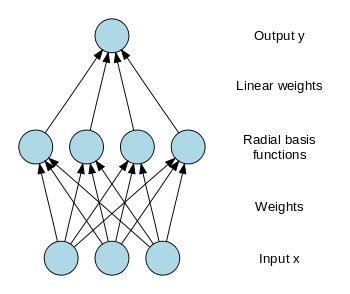
\includegraphics[scale=0.6]{rbf}
\par\end{centering}
\caption{Estructura de las capas de una red neuronal de funciones de base radial.}
\end{figure}